% !TEX encoding = UTF-8 Unicode
\documentclass[12pt,openany, oneside, a4paper,brazil]{abntex2}
\usepackage{indentfirst}
\usepackage[utf8]{inputenc}
\usepackage[T1]{fontenc}
\usepackage{lmodern} %fonte
\usepackage{lastpage} %ficha catalografica
\usepackage[num, overcite]{abntex2cite}
\citebrackets[]
\setlength{\parskip}{0.75cm} % tente também \onelineskip

\titulo{Ferramenta para detecção de padrões de botnet baseado em algoritmos de agrupamento de aprendizagem de máquina}
\autor{Jonas Rocha Lima Amaro \and Yago Guimarães Coimbra}
\data{\today}
\instituicao{Instituto Militar de Engenharia}
\local{Rio de Janeiro}
\tipotrabalho{Projeto de Fim de Curso}
\orientador{Sergio dos Santos Cardoso Silva}
\preambulo{Trabalho Apresentado ao Curso de Engenharia de Computação do Instituto Militar de Engenharia como Verificação Especial do Projeto de Fim de Curso.}

\renewcommand{\imprimircapa}{
	\begin{capa}
		\center
		\large{\textbf{ MINISTÉRIO DA DEFESA\\
			EXÉRCITO BRASILEIRO\\
			DEPARTAMENTO DE CIÊNCIA E TECNOLOGIA\\
			INSTITUTO MILITAR DE ENGENHARIA\\
			ENGENHARIA DE COMPUTAÇÃO - SE/8\\
		}}
		\vspace{5cm}
		\imprimirautor\\
		\vspace{5cm}
		\large{\textbf{\imprimirtitulo}}\\
		\vspace{5cm}
		\imprimirlocal\\
		2016

	\end{capa}
}


\begin{document}
\imprimircapa
\imprimirfolhaderosto{}
\begin{fichacatalografica}
	\begin{tabular}{@{\hspace{0cm}}p{14.8cm}}
	c2014\\
	\\
	\imprimirinstituicao\\
	Praça General Tibúrcio, 80 - Praia Vermelha\\
	Rio de Janeiro - RJ \hspace{1.5cm} CEP: 22290-270\\
	\\
	Este exemplar é de propriedade do \imprimirinstituicao, que poderá incluí-lo em base de dados, armazenar em computador, microfilmar ou adotar qualquer forma de arquivamento.\\
	\\
	É permitida a menção, reprodução parcial ou integral e a transmissão entre bibliotecas deste trabalho, sem modificação de seu texto, em qualquer meio que esteja ou venha a ser fixado, para pesquisa acadêmica, comentários e citações, desde que sem finalidade comercial e que seja feita a referência bibliográfica completa.\\
	\\
	Os conceitos expressos neste trabalho são de responsabilidade dos autores e do orientador.\\
	\\
	\\
	\\
	\end{tabular}

	\small
	\begin{center}
	\begin{tabular}{|cp{13cm}|} \hline
		\hspace{1.3cm} & \\
		& Amaro, Jonas e Guimarães, Yago \\
		\hspace{0.2cm} S586d & \hspace{0.3cm} \imprimirtitulo{} / \imprimirautor. - \imprimirlocal: \imprimirinstituicao, 2016. \\
		& \\
		& \hspace{0.65cm} \pageref{Lastpage}f. : il., graf., tab. : -cm. \\
		& \\
		& \hspace{0.6cm} \imprimirtipotrabalho{} - \imprimirinstituicao \\
		& \hspace{0.6cm} \imprimirorientadorRotulo: \imprimirorientador.\\
		& \\
		& \hspace{0.6cm} 1 - Botnets \hspace{0.1cm} 2 - Clustering\\
		
		& \\ 
		& \hspace{9.75cm} CDU 631.317.35 \\
		\hline
	\end{tabular}
	\end{center}
\end{fichacatalografica}
\begin{folhadeaprovacao}
	\begin{center}
		{\ABNTEXchapterfont\large\imprimirautor}

		\vspace*{\fill}\vspace*{\fill}
		\begin{center}
			\ABNTEXchapterfont\bfseries\Large\imprimirtitulo
		\end{center}
		\vspace*{\fill}
		
		\hspace{.45\textwidth}
			\begin{minipage}{.5\textwidth}
		    	\imprimirpreambulo
		    \end{minipage}
		\vspace*{\fill}
	\end{center}

	Trabalho aprovado. \imprimirlocal, \imprimirdata:

	\setlength{\ABNTEXsignwidth}{10cm}
	\assinatura{\imprimirorientador{} - D.Sc., do IME \\ Orientador}
	\assinatura{Raquel Coelho Gomes Pinto - D.Sc., do IME}
	\assinatura{Julio Cesar Duarte - D.Sc., do IME}

	\begin{center}
		\vspace*{0.5cm}
		{\large\imprimirlocal}
		\par
		{\large\imprimirdata}
		\vspace*{1cm}
	\end{center}
\end{folhadeaprovacao}
\begin{resumo}
	Resumo em pt

	\vspace{\onelineskip}
	\noindent
	\textbf{Palavras-chave}: botnets, clustering.
\end{resumo}

\begin{resumo}[Abstract]
	\begin{otherlanguage*}{english}
		Abstract in English

		\vspace{\onelineskip}
		\noindent
		\textbf{Keywords}: botnets, clustering.
	\end{otherlanguage*}
\end{resumo}
\listoffigures*
\cleardoublepage
\listoftables*
\cleardoublepage
\begin{siglas}
	\item[C\&C] Comando e Controle
	\item[IRC] \textit{Internet Relay Chat}
	\item[HTTP] \textit{HyperText Transfer Protocol}
\end{siglas}
\begin{simbolos}
	\item[$ \Gamma $] Letra grega Gamas
\end{simbolos}
\tableofcontents*

\textual

\chapter{Introdução}
O espaço cibernético sofre com um crescente número de ataques maliciosos. Esse fato faz com que a pesquisa na área de defesa cibernética ganhe muita importância. Ademais, novas formas de ataques cibernéticos são criadas e antigas são atualizadas, dificultando o objetivo de livrar nossas máquinas de qualquer ameaça \citep{bharathula2016equitable}. Uma dessas formas de ameaças, responsável por grande parte dos ataques em larga escala pela Internet atualmente, é formada pelas botnets.

As botnets, que são redes formadas por máquinas infectadas por alguma forma de \textit{malware}, apresentaram um elevado crescimento no início do século XXI, se tornando uma das ameaças mais desafiadoras no campo de defesa cibernética \citep{chang2015measuring}. A detecção dessas redes se tornou um tópico muito importante na área de defesa cibernética, devido ao desafio que é realizar essa detecção, pois, as botnets são muito flexíveis e robustas, além de estarem em processo de aprimoramento contínuo \citep{bu2010new}.

Com a necessidade de realizar essa detecção, mesmo com as mudanças realizadas no funcionamento das botnets ao longo do tempo, o emprego de técnicas de aprendizado de máquina é muito promissor, especialmente as técnicas de agrupamento. É esperado que os bots que formam as botnets, tenham comportamento diferente de usuários convencionais, e, dessa forma, espera-se que eles sejam agrupados em grupos menores dos formados pela massa de usuários normais.

Levando em conta essas características, o presente trabalho busca desenvolver uma ferramenta para auxiliar na detecção de botnets, utilizando as informações das consultas ao servidor DNS realizadas na rede através de algoritmos de aprendizado de máquina.

\section{Objetivo}
O objetivo deste trabalho é desenvolver uma ferramenta para auxiliar na detecção de possíveis hospedeiros de bots em uma botnet, reduzindo o trabalho humano utilizado na detecção das botnets. Isso será feito utilizando algoritmos de agrupamento, que utilizarão dados que serão calculados através das informações contidas em consultas de DNS realizadas. 

Além disso, o desempenho dessa ferramenta será avaliado, utilizando as informações do log de DNS dos servidores do IME, para o qual já temos algumas máquinas infectadas previamente mapeadas por inspeção e investigação manuais.

\section{Motivação}
O crescimento e diversificação do uso da Internet, criaram o cenário ideal para o desenvolvimento das botnets, que são consideradas uma das maiores ameaças atuais na área de segurança da informação \citep{ji2008botnet}. 

Esta ameaça requer uma atenção especial, principalmente no âmbito militar, devido à aplicação que as botnets podem ter no contexto de defesa cibernética, permitindo que os atacantes inutilizem servidores do inimigo e/ou coletem informações confidenciais.

A detecção das botnets é um grande desafio, pois os atacantes estão sempre aprimorando o funcionamento dos bots, e com isso, os mecanismos atuais muitas vezes falham ao detectar novas implementações de botnets. Isso motivou o uso de algoritmos de agrupamento para serem utilizados na detecção de botnets, de forma que a ferramenta seja capaz de detectar inclusive botnets que sejam desconhecidas.

Por esses motivos, torna-se muito clara a necessidade da criação de uma ferramenta que permita facilitar o trabalho de detecção de novas botnets, não previstas pelas ferramentas atuais, já que novas botnets só poderiam ser identificadas por inspeção manual, que é um processo bastante complexo devido à enorme quantidade de informações presentes em uma rede.

\section{Justificativa}
A justificativa desse trabalho é contribuir para a área de defesa cibernética, uma área de interesse do IME e do Exército Brasileiro (EB), uma vez que em 2008 foi aprovado um decreto que determina essa área como um dos setores prioritários para o EB. apoiando à pesquisa com o conhecimento de características de consultas de DNS que podem ser relevantes para realizar a detecção de botnets. Além disso, a ferramenta pode ser utilizada pelo Centro de Defesa Cibernética (CDCiber) ou servir como um módulo de um sistema integrado de detecção de botnets \citep{silva2012arquitetura}, auxiliando na investigação de atividades suspeitas nas redes.

\section{Metodologia}
Este trabalho foi dividido em cinco fases principais: estudo teórico, preparação dos dados, implementação dos algoritmos de agrupamento aos dados preparados, breve análise e testes dos resultados e implementação da interface gráfica. 

Na etapa de estudo teórico foi feito um levantamento da funcionalidade das botnets e do funcionamento e aplicações dos algoritmos de aprendizado de máquina, com o objetivo de identificar vulnerabilidades e padrões nas botnets, motivando a seleção de características relevantes dos dados utilizados, de forma a melhorar a performance do algoritmo.

Na etapa seguinte, foi feito um levantamento das características candidatas a serem utilizadas pelo algoritmo da ferramenta. De posse dessas características, foi implementado um programa em C++ para realizar a extração automática dessas características da base de dados que utilizamos.

Na etapa de implementação dos algoritmos de agrupamento aos dados preparados, utilizamos a ferramenta \textit{Scikit-Learn} para desenvolvermos um programa escrito em Python que aplica algoritmos de aprendizado de máquina nas características previamente levantadas.

Posteriormente, foi feita uma breve análise, para identificar as técnicas mais adequadas, possíveis refinamentos na ferramenta e comprovar sua eficiência na detecção de bots.

Por fim, foi implementada uma interface gráfica para facilitar o uso da ferramenta pelos usuários, integrando todos as funcionalidades desenvolvidas em uma aplicação multi-plataforma utilizando a ferramenta \textit{Qt Creator}.

\section{Estrutura}
Este trabalho é composto por sete capítulos, iniciando com esta introdução. No capítulo 2 é feito um estudo teórico sobre botnets para identificar o tipo de \textit{malware} que desejamos identificar. Em seguida, no capítulo 3, é realizado um estudo sobre algoritmos de aprendizado de máquina dando ênfase nos algoritmos de agrupamento, que será a estratégia utilizada neste trabalho. Em seguida, no capítulo 4, são explicados os procedimentos e a motivação que levaram à forma de tratamento dos dados. O capítulo 5 mostra quais foram os resultados preliminares encontrados, fazendo uma análise sobre as características dos grupos formados, mostrando as motivações para os próximos aprimoramentos. No capítulo 6, são mostradas as funcionalidades do sistema desenvolvido com a interface gráfica e como foi feita sua arquitetura. Ao final, no capítulo 7, estão as conclusões que foram obtidas ao longo do desenvolvimento da ferramenta.
\chapter{Botnets}
As Botnets são redes formadas por máquinas infectadas com malware, permitindo que o atacante (\textit{botmaster}) realize diversas atividades criminais remotamente, como roubo de informações, ataques de negação de serviço, envio de SPAM, etc.\cite{silva2013botnets}

Com o crescimento e diversificação do uso da Internet, o meio cibernético se tornou mais relevante e mais atraente para a realização de ataques maliciosos. Isso motivou o crescimento do número de botnets existentes e aumentou o potencial de contaminação das mesmas, além disso, para evitar os mecanismos de detecção existentes, elas se tornaram cada vez mais sofisticadas.

Para que o detector se torne mais robusto, é preciso compreender o funcionamento das botnets e seus objetivos. Esse conhecimento é necessário para entender as configurações existentes nas botnets atuais, além de compreender como essas configurações podem evoluir. De posse desse conhecimento, espera-se que seja possível identificar características relevantes e intrínsecas ao funcionamento das botnets, mesmo quando o \textit{botmaster} estiver tentando evitar os mecanismos de detecção.

\section{Elementos das Botnets}
As botnets apresentam alguns elementos estruturais tipicamente envolvidos, que estão presentes independente do protocolo ou arquitetura utilizada. A Figura \ref{fig:typical_elements} mostra a estrutura desses elementos e como eles se relacionam em uma botnet. Segue uma descrição para cada componente:
\begin{itemize}  
\item Bots: São malwares instalados nos computadores das vítimas que podem realizar as ações maliciosas que o \textit{botmaster} envia através do canal de comando e controle (C\&C). Geralmente, o malware é inicializado quando o hospedeiro inicializa a máquina, porém isso pode ser configurado pelo \textit{botmaster} para dificultar a detecção da atividade maliciosa.
\item Hospedeiros (Zumbis): São as máquinas em que o bot foi instalado, ou seja, infectadas.\cite{puri2003bots}
\item \textit{Botmaster}: é o indivíduo que configura o bot, dissemina e controla a botnet.
\item Canal de Comando e Controle (C\&C): é o meio que o \textit{botmaster} tem para se comunicar com a sua botnet. É a parte chave do funcionamento, pois é necessário para o envio dos comandos de atividade maliciosa aos hospedeiros. Dessa forma, grande parte das características da botnet, como robustez, facilidade de detecção/desativação, estabilidade, etc., são definidas pela forma que a infraestrutura de C\&C está organizada.
\end{itemize}

\begin{figure}
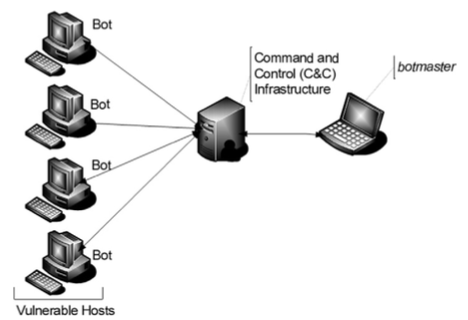
\includegraphics[width=\textwidth]{typical_elements}
\caption[Elementos das botnets]{Elementos das botnets \cite{silva2013botnets}} \label{fig:typical_elements}
\end{figure}

\section{Ameaças e Formas de Defesa}
O crescimento do número de máquinas conectadas constantemente a enlaces de alta velocidade e rodando sistemas com vulnerabilidades consideráveis, criou um ambiente favorável à formação de botnets. Além disso, muitas vezes o bot é transparente ao responsável pela máquina infectada, ou seja, não atrapalha o funcionamento da máquina, fazendo com que a vítima não perceba a infecção e tente combatê-la. Esses fatores, aliados ao enorme potencial de causar danos, fazem com que as botnets sejam um dos maiores desafios de pesquisa em segurança no espaço cibernético atual. \cite{soltani2014survey}

Existem características que tornam o host mais interessante ao \textit{botmaster} como: altas taxas de transmissão, baixos níveis de segurança e monitoração, alta disponibilidade e localização distante (dificultando que as agências reguladoras detectem as atividades, já que os bots estarão espalhados por diversas nações). Esses fatores ajudam o bot a passar desapercebido e a contribuir com maior capacidade de banda ao \textit{botmaster}, facilitando ataques como os de negação de serviço.

Existem duas formas para combater um ataque realizado por botnets: reativamente ou preventivamente. A forma reativa é a mais comum e envolve detectar a existência da atividade maliciosa e reagir ao ataque tentando reduzir o tráfego malicioso para níveis aceitáveis. Uma desvantagem é que o ataque já vai ter sido inicializado quando for detectado, ou seja, já vai haver causado danos antes de ser solucionado. A forma preventiva busca evitar que a botnet possa realizar alguma atividade maliciosa, porém essa atividade não é simples, já que o atacante pode aprimorar seus bots, tornando-os mais sofisticados, exigindo grandes investimentos para manter os recursos de segurança atualizados.

O mecanismo que estamos desenvolvendo é da forma preventiva, já que o algoritmo busca encontrar padrões e identificar possíveis máquinas infectadas por botnets. Tudo isso na fase de disseminação da botnet, ou seja, antes do atacante realizar um ataque, como negação de serviço, por exemplo. Uma característica desejável para um detector é a detecção em tempo real, com o objetivo de minimizar os danos causados e o tempo de reação do \textit{botmaster}. Porém, obter essa característica é um desafio, devido ao grande número de dados que devem ser tratados e analisados. Dessa forma, nosso projeto não fará detecção em tempo real, mas tentará se aproximar disso, utilizando a detecção dos dados coletados ao longo de um dia para detectar bots que atuaram nas últimas 24 horas.

\section{Ciclo de Vida das Botnets}
Na maioria dos casos, existe um ciclo com fases bem definidas de como uma botnet é criada e mantida, a Figura \ref{fig:botnets_lifecycle} mostra essas fases para cada novo hospedeiro que é contaminado.

\begin{figure}
\tikzstyle{block} = [rectangle, draw, text width=9em, text centered, rounded corners, minimum height=4em]
\tikzstyle{line} = [draw, -latex']
\centering
\begin{tikzpicture}[node distance = 4.5cm, auto]
    % Place nodes
    \node [block] (init) {Infecção Inicial};
    \node [block, below of=init] (second) {Injeção Secundária};
    \node [block, right of=init] (connection) {Conexão};
    \node [block, below of=connection] (malicious) {Atividades Maliciosas};
    \node [block, right of=malicious] (update) {Manutenção e Atualização};
    % Draw edges
    \path [line] (init) -- (second);
    \path [line] (second) -- (connection);
    \path [line] (connection) |- +(4,2) |- (connection.east); 
    \path [line] (connection) -- (malicious);
    \path [line] (malicious) -- (update);
    \path [line] (update) -- (connection);

\end{tikzpicture}
\caption[Ciclo de Vida das Botnets]{Ciclo de Vida das Botnets} \label{fig:botnets_lifecycle}
\end{figure}

Na primeira fase, chamada de injeção inicial, o atacante procura vulnerabilidades na máquina do futuro hospedeiro para explorá-las e infecta-lo com o malware, tornando-se um bot em potencial, isso pode ocorrer, por exemplo, através de um download indesejado ou através de um anexo em um e-mail. Após a infecção ser bem sucedida, ocorre a injeção secundária: o host infectado, através do malware inicial instalado, busca em uma rede os reais binários do malware do bot, os quais após baixados e executados concluirão a infecção e tornam o host em um bot real.\cite{feily2009survey}.

Durante a fase de conexão, o bot estabelece conexão com o canal de C\&C, isso se repete sempre que o host é reiniciado, podendo ser considerada uma fase vulnerável já que segue um padrão. Após a efetivação da conexão, o bot se torna ativo na botnet, e passa a realizar os comandos enviados pelo \textit{botmaster} através do canal de C\&C, efetivando as atividades maliciosas solicitadas. A última fase é a de manutenção e atualização, e tem por objetivo manter a botnet ativa e atualizada, já que se o \textit{botmaster} deseja que os bots possam evitar novas técnicas de detecção, adicionar novas funcionalidades ou até mesmo alterar o servidor de C\&C, os binários do programa bot devem ser modificados.

\section{Arquitetura das Botnets}
Existem 4 tipos de arquiteturas para as botnets: centralizada, descentralizada, híbrida e aleatória. 

Na arquitetura centralizada, mostrada na Figura \ref{fig:centralized_architecture} todos os bots se comunicam com um número pequeno de servidores de C\&C, embora ela ofereça vantagens ao \textit{botmaster}, como baixa latência e facilidade de manutenção, ela também torna a botnet bastante vulnerável, permitindo que ela seja desligada após a identificação dos poucos pontos centrais de C\&C. Ela é muito utilizada pelo protocolo IRC (\textit{Internet Relay Chat}), porém pelo fato de tráfego desse protocolo ser incomum e raramente utilizado, ele costuma ser bloqueado, inutilizando a botnet. Por isso, o uso do protocolo HTTP (\textit{HyperText Transfer Protocol}) se popularizou já que ele é muito utilizado, disfarçando as comunicações das botnets.

\begin{figure}
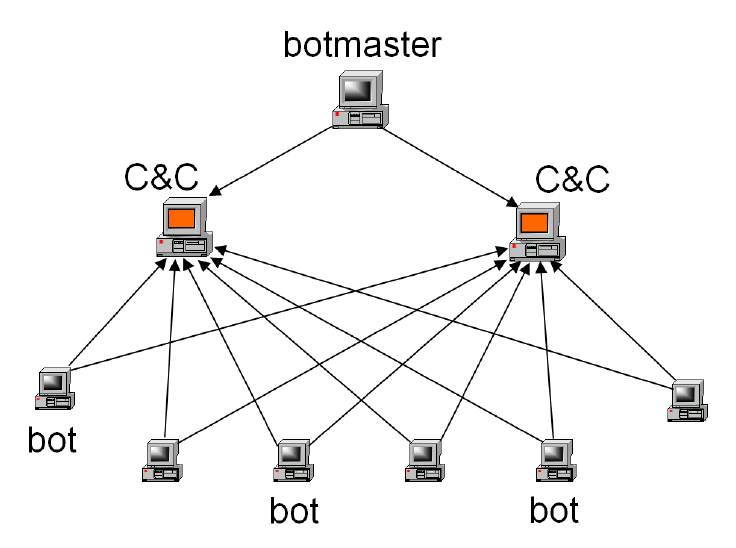
\includegraphics[width=\textwidth]{centralized}
\caption[Arquitetura Centralizada]{Arquitetura Centralizada\cite{wang2010advanced}} \label{fig:centralized_architecture}
\end{figure}

A fragilidade da arquitetura centralizada, motivou o desenvolvimento da arquitetura descentralizada, na qual uma variedade de protocolos P2P (\textit{Peer-to-peer}) é utilizada. A flexibilidade e robustez dessa arquitetura, permite que mesmo que muitos bots sejam desativados a botnet possa continuar funcionando, já que não existem pontos centralizados de C\&C. 

As arquitetura híbridas apresentam características de ambas as arquiteturas centralizadas e descentralizadas, como mostrado na Figura \ref{fig:hybrid_architecture}, na qual os bots são classificados em dois grupos: clientes e servos. Os servos exercem os papéis tanto de clientes quanto servidores, possuindo endereço de IP estático e público para serem acessíveis globalmente, sendo utilizados para repassar os comandos enviados pelo \textit{botmaster}. Os demais bots, são denominados clientes pois não aceitam comunicações de entrada, dessa forma e podem apresentar IP dinâmico, privado ou protegidos por \textit{firewall} para não serem roteados facilmente. Por fim, a arquitetura aleatória é um modelo até agora teórico, no qual o bot não se comunica ativamente com o \textit{botmaster} ou com outros bot, para realizar um ataque o \textit{botmaster} vasculha a rede em busca de um bot para enviar o comando e realizar as atividades maliciosas.

\begin{figure}
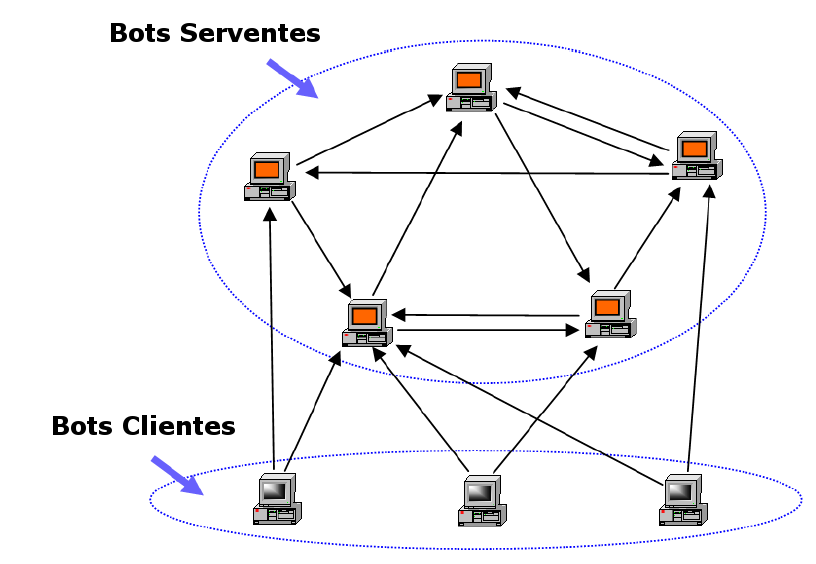
\includegraphics[width=\textwidth]{hybrid}
\caption[Arquitetura Híbrida]{Arquitetura Híbrida\cite{wang2010advanced}} \label{fig:hybrid_architecture}
\end{figure}

\section{Detecção de Botnets}

Existem duas categorias de técnicas para detecção de botnets: \textit{honeynets} e sistemas de detecção de intrusos (IDS). As \textit{honeynets} consistem na criação de redes com a intenção de que elas sejam comprometidas, permitindo que as informações sobre a botnet sejam captadas, por isso elas são consideradas mais efetivas para compreender as características de uma botnet do que a detecção propriamente dita.

A detecção por IDS, pode ser classificada entre duas técnicas: a baseada em assinaturas e a baseada em anomalias. A técnica baseada em assinaturas, consiste em extrair padrões da rede e comparar com um banco de dados onde se encontram os padrões que já foram vistos em botnets, ou seja, ela não permite que novas botnets sejam identificadas e envolve a posse de um banco de dados enorme com o maior número de informações existentes sobre as botnets previamente detectadas. Dessa forma, a técnica baseada em anomalias é a principal área de pesquisa para detecção de botnets, baseando-se em anomalias na rede, como alta latência, aumento no tráfego ou uso de portas incomuns para detectar a presença de bots na rede.

As técnicas baseadas em anomalias, podem ser baseadas no host, onde cada máquina possui uma ferramenta de monitoração instalada (o que não é muito escalável), e tem seu comportamento analisado para verificar a existência de atividades suspeitas. Além disso, a análise pode ser baseada na rede, ativa (que possuem a grande desvantagem de aumentar o tráfego da rede ao injetar pacotes com a finalidade de examinar se um cliente é humano ou um bot) ou passivamente, sendo esta última a forma de detecção mais utilizada e pesquisada atualmente.

A monitoração passiva de uma rede consiste em analisar o tráfego da rede buscando por comunicações suspeitas que podem ter sido enviadas pelos bots ou canais de C\&C. Essa monitoração é possível pois os bots de uma mesma botnet costumam apresentar padrões de comunicação, já que eles são pré-programados pelo mesmo \textit{botmaster} para entrar contato com o servidor de C\&C.

Para que a análise do tráfego seja viabilizada, são empregadas diversas técnicas como métodos estatísticos, mineração de tráfego, teoria de grafos, clustering, modelos estocásticos, redes neurais, entre outras.

A detecção de botnets é uma tarefa bastante desafiadora porque os \textit{botmaster}s estão sempre aprimorando os bots, tornando os mais difíceis de serem detectados. Por exemplo, as primeiras detecções buscavam mensagens suspeitas nos conteúdos da mensagem, afim de evitar isso os \textit{botmaster}s passaram a utilizar criptografia tornando essa técnica de detecção obsoleta. Outra dificuldade para algoritmos de clustering é que podem ser evitados usando técnicas de randomização nas comunicações e atribuição de tarefas diferentes para os bots.


\chapter{Conclusão}

Os clientes IP foram modeladas segundo algoritmos de agrupamento apresentados no Capítulo \ref{ch:machine} utilizando características levantadas no Capítulo \ref{ch:data_preparation}. Essas caracterísiticas evidenciam os bots se considerando a arquitetura das botnets estudada no Capítulo \ref{ch:botnet}. Dessa forma foi desenvolvido uma ferramenta de apoio à decisão na detecção de bots em log DNS a qual as especificações do caso de uso e as janelas de diálogo foram apresentadas no Capítulo \ref{ch:tool}

A primeira contribuição evidente do trabalho foi próprio desenvolvimento da ferramenta de apoio a decisão que reduz o domínio de análise do usuário através dos algoritmos de agrupamento e permite a visualização dos dados seguindo nos eixos as características previamente levantadas como relevante

Além disso, como contribuição de conhecimento pode-se ressaltar a análise da variação da função custo do modelo gerado pelo K-Médias a cada centroide adicionado ao modelo. Percebeu-se que o Método \textit{Elbow} não é satisfatório para essa análise.

Como alternativa para a descoberta da quantidade centroides foi implementada uma solução de visualização dos dados que permite resgatar as informações de cada ponto escolhido. Essa solução ainda não se mostrou a melhor quando aplicada na base de dados conhecida, mas se mostrou muito útil também para detectar pontos que fogem do padrão mais comum.

Foi feita uma análise no log DNS do IME de 12 de março de 2012 e foi alcançado um resultado satisfatório no qual duas das três máquinas suspeitas já conhecidas estavam presentes no menor grupo.

Como já salientado, a complexidade do algoritmo de Agrupamento por Aglomeração é alta, por isso é importante manter um \textit{cache} dos resultados computados pelo algoritmo para que a troca da quantidade de grupos não apresente a demora de uma primeira contrução da hierarquia dos grupos.

Após uma breve comparação dos dados normalizados contra os não-normalizados, percebeu-se o esperado, é melhor trabalhar com dados normalizados. O resultado era esperado pois, algumas características geram números de ordem muito maior do que a maioria e ainda apresentavam grandes diferenças entre si. Para o algoritmo corria-se o risco haver grupos separados por essa distância relativa.

Apesar desse trabalho ter realizado uma análise, o que inclusive foge um pouco do escopo do projeto, espera-se que em trabalhos futuros as análises com outros dados sejam realizadas. Além disso, espera-se um estudo qualitativo das características implementadas um bom trabalho para o log DNS utilizado, mas não necessariamente se comportará bem com todo tipo de fluxo no log DNS. Espera-se também que seja estudado o algoritmo de agrupamento aglomerativo, o qual foi integrado ao trabalho mas não foi teve resultados analisados. Outros algoritmos devem ser analisados, para validar a solução e garantir o pleno apoio à decisão que esse trabalho se propõe.

\postextual
\bibliography{refs}
\end{document}